\chapter{Metodologie}
\label{chap:metodologie}
L’obiettivo di questo documento è confrontare in modo critico ed esplicito i diversi protocolli di QKD descritti all’interno dello stesso.\\
% aggiungere descrizione delle dimensioni di confronto e come le abbiamo determinate + una possibile dimensione extra è se esistono o meno applicazioni/implementazioni simulate/ implementazioni reali dei protocolli
Al fine di raggiungere gli scopi sopracitati, la nostra metodologia di analisi prevede di:
\begin{enumerate}
    \item illustrare i funzionamenti dei protocolli di QKD BB84, E91, B92 e SARG04 nel capitolo \ref{chap:protocolli_qkd};
    \item effettuare un confronto esplicito dei succitati protocolli di QKD nel capitolo \ref{chap:confronto_esplicito} per mezzo di tabelle facilmente consultabili che fungono anche da tassonomia;
    \item esplicitare considerazioni di natura tecnico-pratica sull'impiego dei succitati protocolli di QKD nel capitolo
    \ref{chap:confronto_esplicito}.
\end{enumerate} 
Relativamente al confronto esplicito, esso sarà costruito sulla base delle seguenti dimensioni di comparazione:
\begin{enumerate}
    \item principio quantistico di funzionamento;
    \item polarizzazione dei fotoni;
    \item numero di stati;
    \item vulnerabilità rispetto agli attacchi descritti nel capitolo \ref{chap:background};
    \item presenza di implementazioni reali (sperimentali o industriali) e/o simulate.
\end{enumerate} 
Ciascuna di queste dimensioni di comparazione, stabilite perché largamente utilizzate in letteratura per confrontare protocolli di QKD, saranno brevemente descritte nelle sezioni sottostanti.

\section{Principio quantistico di funzionamento}

I protolli di QKD basano il proprio funzionamento su uno dei due principi cardine della meccanica quantistica: il principio di indeterminazione di Heisenberg e il quantum entanglement.

L'idea dei protocolli che usano il principio di indeterminazione di Heisenberg è che un \textit{eavesdropper} non può misurare lo stato di fotoni che vengono inviati sul canale di comunicazione senza disturbarne lo stato e, quindi, senza essere scoperti \cite{survey_prominent_qkd}.

L'idea dei protocolli che si basano su quantum entanglement è che le due parti della comunicazione ricevano fotoni "entangled". Ognuna delle due parti sceglie delle basi casuali per misurarli. Per ogni base scelta sia dal mittente che dal destinatario dei fotoni, gli stati letti devono essere opposti. Gli stati letti in corrispondenza di una stessa base possono essere interpretati come due stringhe binarie complementari: una di queste due stringhe può essere utilizzata come chiave segreta di comunicazione \cite{survey_prominent_qkd} \cite{survey_qc}.

\section{Polarizzazione dei fotoni e numero di stati}

Abbiamo visto al capitolo \ref{chap:background} la necessità di scegliere delle basi per rappresentare l'informazione (e successivamente leggerla). Il numero di stati non è altro che il numero totale di possibili polarizzazioni che può assumere un fotone e, conseguentemente, il numero di vettori dell'unione delle basi scelte. Per esempio, il protocollo BB84 prevede quattro stati di polarizzazione che corrispondono a quattro vettori di base: un vettore a 0 gradi e un vettore a 90 gradi (base rettilinea), un vettore a 45 gradi e un vettore a 135 gradi (base diagonale) \cite{survey_qc_qkd} \cite{survey_qkd} \cite{security_individual_realistic_qkd} (per maggiori dettagli, si veda il capitolo \ref{chap:protocolli_qkd}). Quanto spiegato è mostrato in figura \ref{fig:ortobasis} e si può notare con facilità come gli stati entro la stessa base siano ortogonali.

%\section{Polarizzazione dei fotoni}

%Questa dimensione indica se gli stati di polarizzazione usati sono ortogonali. Per esempio, BB84 ha due coppie di stati di polarizzazione: orizzontale (0°) e verticale (90°), diagonale a 45° e diagonale a 135° \cite{survey_qkd}. Si vede quindi come questi stati siano ortogonali a coppie, come mostrato in Figura \ref{fig:ortobasis}.

\begin{figure}[h]
    \centering
    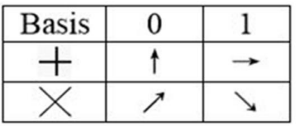
\includegraphics[width=10cm]{immagini/ortobasis.png}
    \caption{I quattro diversi stati di polarizzazione dei fotoni nel protocollo BB84. La base rettilinea (prima riga) e la base diagonale (seconda riga) formano due basi di stati ortogonali \cite{survey_qc_qkd}.}
    \label{fig:ortobasis}
\end{figure}

\section{Vulnerabilità rispetto ad attacchi noti}

Ogni algoritmo presentato può essere suscettibile a qualche attacco e da tale suscettibilità dipende la sicurezza del protocollo di QKD. Pertanto, per un progettista risulta fondamentale conoscere le vulnerabilità dei protocolli che adotterà.

\section{Presenza di implementazioni reali e/o simulate}

I protocolli di QKD, per essere effettivamente testati in molteplici campi di applicazione e sotto svariate condizioni di impiego, necessitano di essere implementati. Pertanto, i protocolli di QKD analizzati nel documento saranno classificati anche in base alla presenza in letteratura di articoli che attestino l'implementazione di tali protocolli in ambienti reali e/o simulati.